\section{Proposed Research}
\label{sec:proposedresearch}

At the best of our knowledge there are not, out there, OpenMP data race
detectors that guarantee low runtime and memory overhead while maintaining
high precision and accuracy.
%
This motivate the need for better data race detection techniques and tools for
structured parallel programming paradigms.
%
As claimed in \S~\ref{sec:introduction}, we propose several different
contributions to obtain a better data race detection tool for OpenMP programs.
%
In the remainder of this section I will discuss and detail our proposed
contributions and how the combination of them helps to obtain a better OpenMP
data race detector.

\textbf{Sequential Blacklisting:} We exploit OpenMP's structured parallelism
to identify guaranteed sequential regions within OpenMP code.
%
Such analysis would be difficult to conduct in the context of unstructured
parallelism (e.g., PThreads).
%
Figure~\ref{fig:nested} shows an example of OpenMP parallel and nested
parallel regions.
%
As we can see, the parallel regions are alternated by the solely main thread
execution.
%
The code executed by the main thread is sequential and cannot race with any
other threads existing in a parallel region.
%
Therefore, the instructions executed by the main thread during its sequential
execution can be excluded from the runtime analysis reducing the overhead.

\begin{figure}
  \centering
  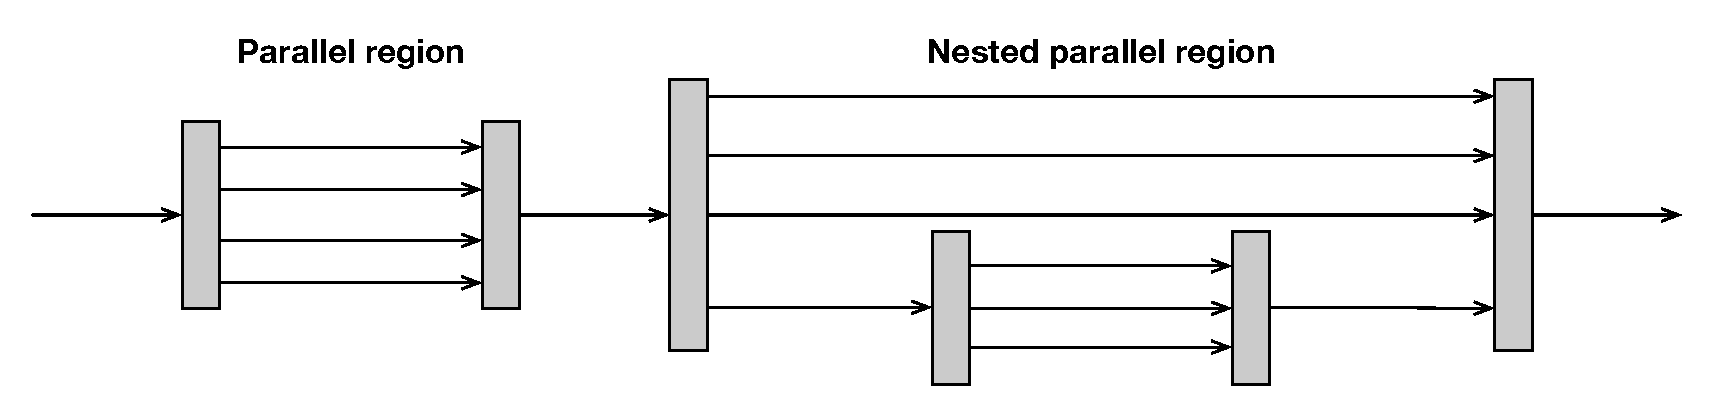
\includegraphics[width=0.95\textwidth]{figures/nested_parallelism}
  \caption{OpenMP nested parallelism}
  \label{fig:nested}
\end{figure}

\textbf{Data Dependency Analysis:} We identify and suppress race free parallel
loops from race checking.
%
Listing~\ref{code:example01} shows an example of two parallel for-loops.
%
The first one is easily and automatically parallelizable, the array will be
divided in different chunks and each of them will be assigned to different
threads.
%
However, the second parallel for-loops has a data dependency in the array
accesses, which will introduce a data race when the array's chunks are
assigned to different threads.
%
Indeed, it may happen that two threads will access the same locations
simultaneously without any synchronization mechanism.
%
The OpenMP compiler do not apply any check and will parallelize both loop in
the same way.
%
We introduce a data dependency analysis at compiling time that identify loops
with and without dependencies.
%
The firsts will be blacklisted and excluded by the runtime analysis since race
free, the seconds instead will be checked at runtime.

\begin{wrapfigure}{L}{0.37\textwidth}
  \vspace{-2ex}
  \begin{lstlisting}[language=C++, caption=OpenMP loops with and without loop-carried data dependency., label=code:example01]
  #pragma omp parallel for
  for(int i = 0; i < N; i++) {
    a[i] = a[i] + 1;
  }

  #pragma omp parallel for
  for(int i = 0; i < N; i++) {
    a[i] = a[i + 1];
  }
  \end{lstlisting}
\end{wrapfigure}

\textbf{\archer v1:} The two previous static analysis techniques and an
instrumented version of the OpenMP runtime make the first version of the
OpenMP data race detector \archer.
%
The static analyses will be implemented as a LLVM/Clang passes and integrated
in the compilation process.
%
We will annotate the OpenMP runtime to communicate the \tsan about the
happens-before relations between threads in presence of unknown
synchronization mechanisms.
%
For example, OpenMP barriers and OpenMP critical section are unknown to the
\tsan runtime, which would make it reports false positives.
%
This first version of \archer is the initial step towards low overhead data
race detector for large OpenMP applications, and it would also allow us to
evaluate the benefits of the static analyses in terms of both overheads
reduction, and precision and accuracy of the data race detection process.

\textbf{Clock-less runtime algorithm:} We propose a new data race detection
algorithm that, differently from past and modern Pthreads data race detection
techniques usually based on vector and lamport clocks, exploits the structured
parallelism of parallel programming models, such as OpenMP, to guarantee high
an equivalent or better data race detection precision and accuracy using less
runtime and memory resources.
%
In OpenMP the concurrency structure generated by its fork-join model is much
simpler than other programming model such as Pthreads.

To highlight the well-structured concurrency model of an OpenMP program
consider the example show in figure~\ref{fig:example01}.
%
The example shows a main thread~\footnote{A thread is represented as a
  circle.} that spawns a parallel region of two threads.
%
After that, each thread will be creates its own nested parallel regions, which
after their execution-life will join to a single thread, and so on for each
region, until they join again to the main thread.
%
Differently from the Pthreads programming models, in OpenMP the main thread
(or in general the forking thread) will be always part of the parallel region
generated, and it will do the same work as the others newly created threads.
%
This emphasize the concurrency model of the threads within a parallel region
and threads across parallel regions.
%
In fact, in OpenMP two threads can race within a same parallel regions (e.g.\
thread 3 and 4) or across parallel regions (e.g.\ thread 3 and 5), but two
threads can not race if they belong to two consequent parallel regions (e.g.\
thread 3 and 9).
%
Threads that belongs to two consequent parallel regions are not concurrent
since there is always a join point that separate them, furthermore in OpenMP,
at the end of each parallel region there is an implicit barrier which
synchronize all the threads before starting the next parallel task.
%
We base our idea of data race detection to these facts, and exploit an
existing thread labeling approach for
fork-join~\cite{Mellor-Crummey:1991:ODD:125826.125861} models to quickly
identify if two threads are concurrent.
%
In this way, we can limit the data race detection only to the concurrent
threads~\footnote{A common happens-before algorithm based on vector clocks
  would perform a race check also on non-concurrent threads, because of its
  lack of knowledge on the concurrency structure of the OpenMP program.}.

We formally define the concurrency structure of OpenMP from the point of view
of race checking.
%
To the best of our knowledge the OpenMP concurrency model has never been
formally documented.
%
We define a state machine and a set of transition rules that model the
behavior of an OpenMP program.                            
%
The appendix~\ref{sec:appendixa} shows the formal definition of the state
machine.
%
We abstract away from data state as much as possible, using uninterpreted
functions to occasionally bridge the gap.
%
The transition system can fire, for any thread, any rule at any point changing
the state of the system.
%
Moreover, it can also fire the ``RaceCheck'' rule at any point of the state
machine execution, flagging the existence of a race.

The transition system is an ideal state machine that guarantees to detect
every race present in an OpenMP program, without reporting any false positive.
%
From the formal point of view, the transition system is a machine with
infinite memory and in fact it keeps track of every memory access performed by
any thread in the system.
%
This approach would not be feasible in the real-world since the runtime and
memory resources are limited, but most importantly because our main goal is to
obtain a low runtime and memory overhead data race detection algorithm.
%
Even though the state machine is an ideal system, it allows to model all the
corner cases in the OpenMP race-checking problem and design a real better
algorithm that guarantee correctness and soundness.

We believe that the transition system can help to design a precise and fast
data race detection algorithm.
%
We intend to implement an algorithm that at runtime models the concurrency
structure of the parallel regions of an OpenMP program.
%
The concurrent model of the program will be stored in a lock-free and fast
data structure~\cite{5871597, Matveev:2015:RLS:2815400.2815406} that can
be concurrently read and written by multiple threads.
%
Furthermore, we will rely in another lock-free and fast data structure to
maintain a smaller representative set of memory accesses performed by the
threads.
%
We plan to perform the data race detection check at every barrier checkpoint.
%
This will limit the number of race checks performed during the program
execution, differently from vector-clock techniques that generally perform the
check at every memory accesses.
%
The real race-check is illustrated by the ``RaceCheck'' rule in
appendix~\ref{subsec:sosrules} on the smaller set of memory accesses.
%
The OpenMP Tools Application Programming Interfaces (OMPT)~\cite{ompt}
implemented by the OpenMP runtime provides all the information to build the
concurrency structured of an OpenMP program at runtime.
%
We will indeed based our implementation on the OMPT API guaranteeing a
standard and portable solution of the data race detection algorithm.

\begin{wrapfigure}{R}{0.5\textwidth}
  \centering
  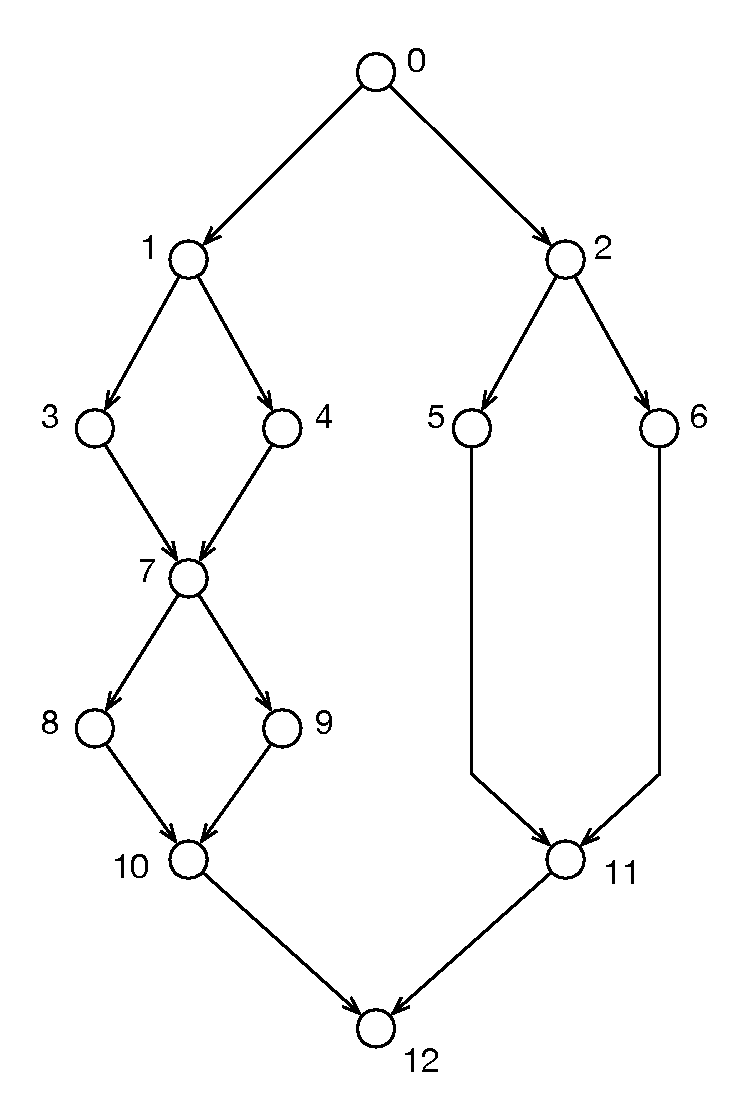
\includegraphics[width=0.45\textwidth]{figures/example01}
  \caption{Structure of an OpenMP program with nested parallelism.}
  \label{fig:example01}
\end{wrapfigure}

\textbf{\archer v2:} The second version of \archer will embed both static
analyses and the runtime analysis technique for data race detection of
structured parallelism.
%
We plan to integrate \archer in the LLVM/Clang compiler infrastructure and
guarantee the same ease to use that characterize most LLVM tools.
%
In fact, we will provide a new compilation flag (i.e. ``-archer'') that will
instrument the OpenMP program at compile time and will link it against the
\archer runtime library.
%
The program can then be executed as usual, while the \archer runtime library
will perform the data race detection providing at the end of the execution a
detailed report about the detected races.

%%% Local Variables:
%%% mode: latex
%%% eval: (flyspell-mode 1)
%%% TeX-master: "root.tex"
%%% End:
